\documentclass[a4paper, 12pt]{report}

\usepackage[pagestyles]{titlesec}
\usepackage[backend=bibtex]{biblatex}

\usepackage[printonlyused]{acronym}
\usepackage{amsmath}
\usepackage{graphicx}
\usepackage{float}
\usepackage{array}
\usepackage[margin=1in]{geometry}

\title{Mars Sample-Return Rover \\
\large ENPM 662 Final Project}
\date{December 2020}
\author{Robert Vandemark \and Diane Ngo}

\addbibresource{references.bib}
\nocite{*}

\acrodef{SRR}[SRR]{\emph{Sample-Return Rover}}
\acrodef{4DOF}[4DOF]{\emph{Four Degrees of Freedom}}

\titleformat{\chapter}[block]{\Huge\bfseries}{\thechapter}{1em}{\Huge\bfseries}

\titlespacing{\chapter}{0pt}{0pt}{10pt}
\renewcommand{\baselinestretch}{1.15}

\begin{document}
	
	\setcounter{page}{1}
	\maketitle
	
	\tableofcontents
	\newpage
	
	\chapter{Abstract}
	Throughout recent decades, the topic of space exploration is desirable towards scientists and researchers. Mars is the nearest planet that is possible to explore in great detail. There are many challenges pertaining to exploring unknown territory, through long distance, and difficulty of remotely operating robots. NASA’s approach to exploring and researching Mars was through the Sample Return Rover, created in 1997 by the JPL Jet Propulsion Laboratory. The scope of this project focuses on the Mars Rover, its wheel-slip detection (traction control), and path-planning towards a desired object. 

	\chapter{Introduction}
	The Mars Rover is a Sample Return Rover designed by the JPL NASA Laboratory. It consists of a chassis with a central revolute joint on both the left and right sides of the robot. The central revolute joint is connected to two links (on each side),  for the front and rear wheels. Each respective link is connected to another link downward that is connected to a wheel. The front links are revolute so that the robot can turn left and right. Note that the original paper is based off of the Curiosity Rover, which has six wheels. The focus on this paper will be on the Sample Return Rover, which has four wheels. 

Primitive designs of this robot had a large amount of damage to the rover’s wheels. This wheel damage reduced the longevity of the Mars Rover mission by a great amount. NASA had to counteract this damage through researching the cause of the wheel damage. The rover did not properly avoid terrain obstacles nor did it deal with traction loss. The goal for this project is to recreate the traction control algorithm and simulate the results. The algorithm for the traction control is a velocity-based algorithm. One wheel on the rover will be rotating much faster than the others. The traction control system then applies a brake to that wheel to reduce its slip and then reducing wheel slip.


%Here is some example text, which lives in the file \textit{srr\textunderscore ws/src/srr/latex/ traction\textunderscore control/sections/introduction/introduction.tex}, and is made an input in \textit{srr\textunderscore ws/src/srr/latex/traction\textunderscore control/traction\textunderscore control.tex}. LaTeX uses a bunch of macros to stylize and simplify writing reports like these, like how the filepaths were italicized with the \textbf{\textbackslash textit} command. There's a text environment, where this text is being written in, and then there's a math environment, which can format stuff to be all pretty such as:
%
%\begin{equation}\label{traction_control:intro:quad}
%	x_{1,2} = \frac{-b \pm \sqrt{b^{2} - 4ac}}{2a}
%\end{equation}
%
%And then you can reference the super important equation \eqref{traction_control:intro:quad} by naming it, so you never have to keep track of which number equation it is, etc. \\
%
%Ending a line with \text{\textbackslash \textbackslash} will force a new line, like just above this sentence. Also, here's a figure with a centered caption below it:
%
\begin{figure}[htbp]
	\centering
	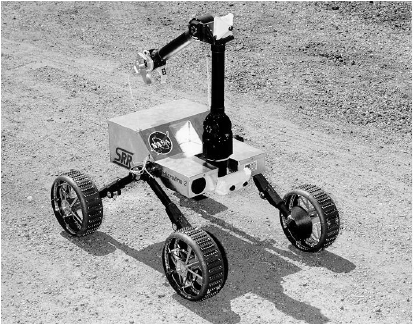
\includegraphics[width=.9\textwidth]{sections/introduction/images/srr.png}
	\caption{An Early Version of the Sample-Return Rover}
\end{figure}

%Again, it's numbered automatically, so we don't have to change that if we decide to move stuff around. If we decide to change the style later, we just have to renew commands and recompile, we don't have to change the content of these files, etc. There are even likely premade IEEE stylesheets that can be imported and automatically applied to everything in this document. \\
%
%Press the green button at the top to compile the main .tex file, TeXstudio will render a preview of the document for you. You can right click on the PDF preview and click "Go to Source" if you want to open the location of whatever it is you clicked on, if you see a typo you want to change quickly, etc. Try it with this paragraph or the figure.


	\chapter{Robot Design}
	\noindent
The robot base comprises of four legs, with two on each side that are concentric. On either side, two of the legs are connected via a revolute joint and is concentric. The front wheels have a revolute joint connected to the wheels so that the robot can steer left or right. To have the robot at the same height, the rear wheels have the same joint however it is fixed. The robot arm that is attached has four degrees of freedom.\\

Modeling the robot is split into the vehicle and arm separately. With this method, both models can be configured and tested properly in Gazebo in order to use tele-op on individual joints. Figure~\ref{sample_return_rover:robot_design:srr_cad} shows the rover modeled in SolidWorks. Table~\ref{table:1} lists the dimensions of the robot and links. Figure~\ref{sample_return_rover:robot_design:arm_model} and Figure~\ref{sample_return_rover:robot_design:arm_side} are images of the arm for reference.

\begin{table}[h]
\begin{center}
	\begin{tabular}{|c|c|} 
		\hline 
		\textit{Link} & \textit{Length} \\
		\hline
		Chassis Length & 18in \\
		Chassis Width & 12in \\
		Chassis Max Height & 7in \\
		Leg from Center Joint & 8.6in \\
		Length of Steering Link & 5.25in \\ 
		Wheel Diameter & 7.5in \\
		Wheel Track & 19.3in \\
		Wheelbase & 13.9in \\
		\hline
	\end{tabular}
	\caption{\label{table:1}Table of Dimensions of the Rover}
\end{center}
\end{table}

\begin{figure}[h]
	\centering
	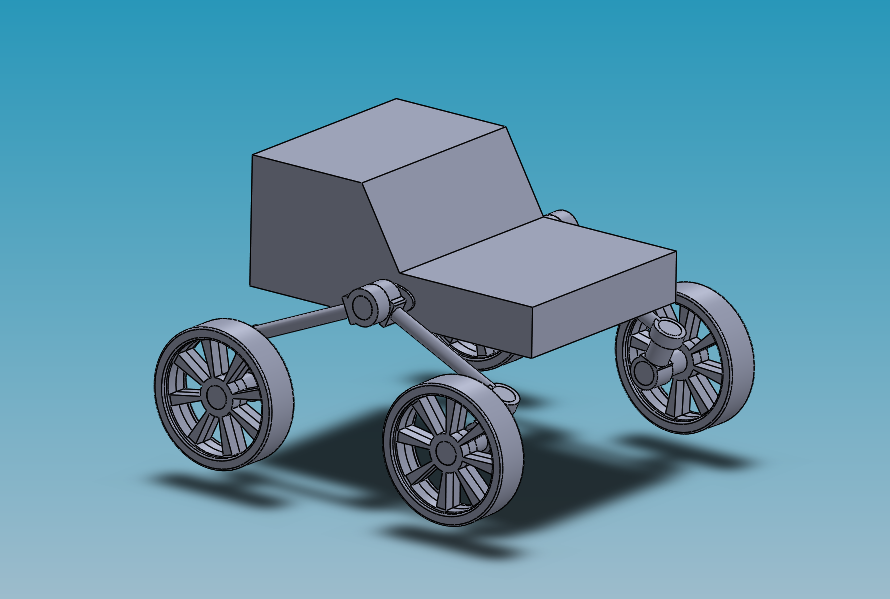
\includegraphics[scale=0.45]{sections/robot-design/images/SRR_model.png}
	\label{sample_return_rover:robot_design:srr_cad}
	\caption{Sample Return Rover in SolidWorks}
\end{figure}

\begin{figure}[H]
	\centering
	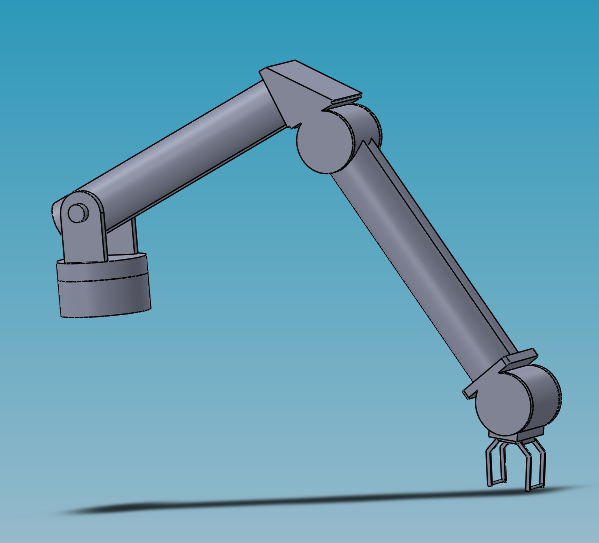
\includegraphics[scale=0.45]{sections/robot-design/images/arm_model.png}s
	\label{sample_return_rover:robot_design:arm_model}
	\caption{Arm Model in SolidWorks}
\end{figure}

\begin{figure}[H]
	\centering
	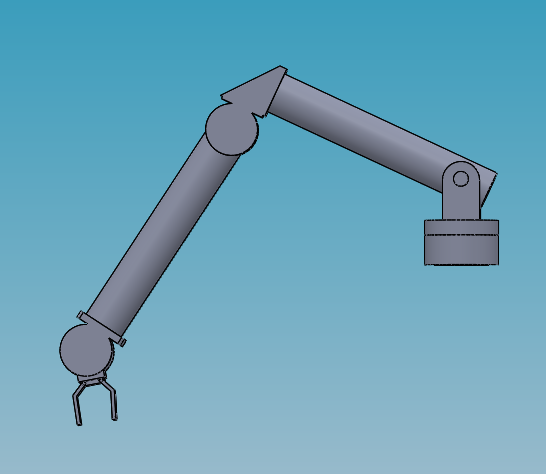
\includegraphics[scale=0.50]{sections/robot-design/images/arm_side.png}
	\label{sample_return_rover:robot_design:arm_side}
	\caption{Side View of Robot Arm}
\end{figure}


	\chapter{Forward Kinematics}
	\section{Vehicle}
The rover uses an Ackermann steering mechanism to be able to navigate, like that seen in Figure~\ref{sample_return_rover:fwd_kin:ackermann}. Unlike the average robotic arm, it is not a serial connection. Forward kinematics cannot be used on a mobile robot. Ackermann steering allows the front wheels to rotate independently, about a common center point. This center point is called the \textit{Instantaneous Center of Curvature} (ICC). In general, it uses a four bar linkage in a trapezoidal shape. However the Curiosity Mars Rover and the Sample-Return Rover does not use this linkage, but the model still holds.

\begin{figure}[H]
	\centering
	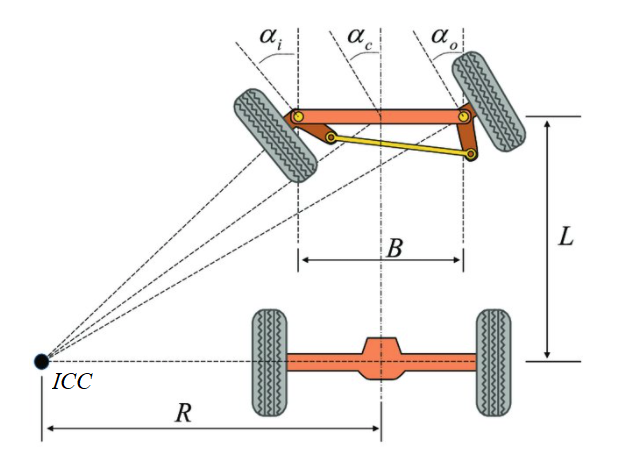
\includegraphics[scale=0.65]{sections/robot-design/images/ackermann_steering.png}
	\caption{Diagram for Ackermann Steering}
	\label{sample_return_rover:fwd_kin:ackermann}
\end{figure}

\section{Arm}
In robotics, forward kinematics is used to find the position and orientation of the robot's end-effector (or gripper) given the joint angles. In this course, joints can have two different types: \textit{revolute} and \textit{prismatic}. A revolute joint rotates about an axis, while a prismatic joint translates linearly along an axis. In serial kinematic chains, such as the arm seen in Figure~\ref{sample_return_rover:robot_design:arm_side}, each coordinate frame assigned to the distal end of a link \textit{i} is dependent on the position and geometry of the $(i-1)^{th}$ joint and link, respectively. The frame \textit{i} resolved in frame \textit{i - 1} represents a combination of a rotation performed by the $(i-1)^{th}$ joint with a successive translation down the length of link \textit{i - 1}. Chaining these homogeneous transformation matrices together results in the transformation of the end-effector in the robot's base frame. \\

The robot arm itself is \ac{4DOF} where each joint is revolute. However, as seen in Figure~\ref{sample_return_rover:robot_design:arm_frames}, there are eight frames in total, because four dummy frames are for Gazebo to properly render in the arm. Its corresponding DH table is shown in Table~\ref{sample_return_rover:robot_design:dh}, and the values for the nonzero static lengths can be seen in Table~\ref{sample_return_rover:robot_design:dh_values}. A list of the links are shown in Figure~\ref{sample_return_rover:robot_design:arm_diagram}. The links \textit{LeftFinger} and \textit{RightFinger} are just there for Gazebo to be able to rotate the end-effector fingers, but they are not used in the DH parameters and table. \\

Note that the arm's home position starts with all angles being at 0, so the arm is fully upward. Each joint has a limit for its range of motion so that the robot does not crash into itself. Equation~\ref{sample_return_rover:robot_design:th1} to \ref{sample_return_rover:robot_design:th4} offer reasonable ranges of allowable motion.

\begin{figure}[htbp]
	\centering
	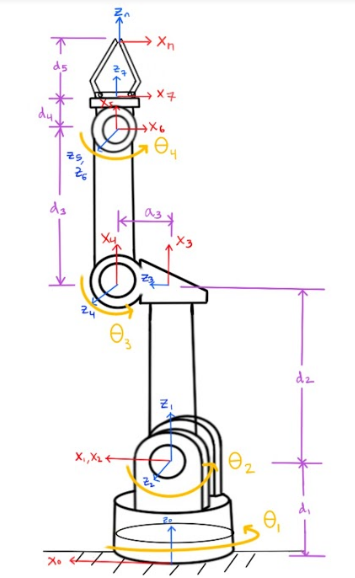
\includegraphics[scale=0.6]{sections/robot-design/images/arm_frames.png}
	\label{sample_return_rover:robot_design:arm_frames}
	\caption{DH Frames of the Arm}
\end{figure}

\begin{figure}[H]
	\centering
	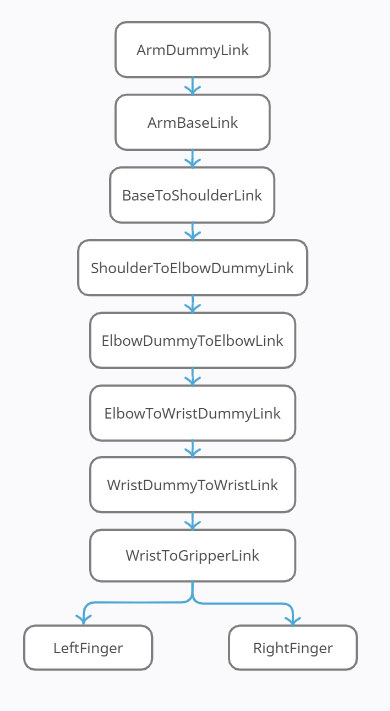
\includegraphics[scale=0.75]{sections/robot-design/images/arm_link_diagram.png}
	\label{sample_return_rover:robot_design:arm_diagram}
	\caption{Flowchart of the Arm Links}
\end{figure}

\begin{table}[htbp]
	\centering
	\begin{tabular}{|c|c|c|c|c|}
		\hline
		\textit{Link i} & \textit{$\theta$} & \textit{d} & \textit{$\alpha$} & \textit{a}\\
		\hline
		1 & $\theta_{1}$ & $d_{1}$ & 0 & 0 \\
		2 & 0 & 0 & -90 & 0 \\
		3 & $\theta_{2}$ - 90  & 0 & -90 & $d_{2}$ \\
		4 & 0  & $a_{3}$ & 90 & 0 \\
		5 & $\theta_{3}$ & 0 & 0 & $d_{3}$ \\
		6 & $\theta_{4}$ - 90 & 0 & -90 & 0 \\
		7 & 0 & $d_{4}$ & 0 & 0 \\
		n & 0 & $d_{5}$ & 0 & 0 \\
		\hline
	\end{tabular}
	\label{sample_return_rover:robot_design:dh}
	\caption{DH Table for the Arm}
\end{table}

\begin{table}[H]
	\centering
	\begin{tabular}{|c|c|}
		\hline
		\textit{Distance between Frames} & \textit{Length} \\
		\hline
		Base to Frame 1 ($d_{1}$) & 2.9in \\
		Frame 2 to Frame 3 ($d_{2}$) & 7.73in \\
		Frame 3 to Frame 4 ($a_{3}$) & 1.76in \\
		Frame 4 to Frame 5 ($d_{3}$) & 8.93in \\
		Frame 6 to Frame 7 ($d_{4}$) & 1in \\
		Frame 7 to Frame n ($d_{5}$) & 1.41in \\
		\hline
	\end{tabular}
	\label{sample_return_rover:robot_design:dh_values}
	\caption{Table of Link Lengths of the Arm}
\end{table}

\begin{equation}\label{sample_return_rover:robot_design:th1}
	\theta_{1} = [-\pi,\; + \pi]
\end{equation}

\begin{equation}\label{sample_return_rover:robot_design:th2}
	\theta_{2} = \left[0,\; +\frac{2\pi}{3}\right]
\end{equation}

\begin{equation}\label{sample_return_rover:robot_design:th3}
	\theta_{3} = [0,\; + \pi]
\end{equation}	

\begin{equation}\label{sample_return_rover:robot_design:th4}
	\theta_{4} = \left[-\frac{2\pi}{3},\; +\frac{2\pi}{3}\right]
\end{equation} \\

One method to start calculating the forward kinematics is to create DH matrices $T^{n-1}_{n}$, which are composed of rotations about the z-axis, translations in the z-axis, rotations about the x-axis, and finally translations in the x-axis. The basic rotation matrix for a rotation about the z-axis with an angle $\theta$ can be shown in Equation~\ref{sample_return_rover:robot_design:rz}, and Equation~\ref{sample_return_rover:robot_design:rx} for rotation about the x-axis by angle $\alpha$. The translation vectors can be seen in Equations~\ref{sample_return_rover:robot_design:dx} and~\ref{sample_return_rover:robot_design:dz} for along the z and x axes by a displacement \textit{d} and \textit{a}, respectively. Using the DH Table, the homogeneous transformation matrices can now be written. The setup for this matrix is seen in Equation~\ref{sample_return_rover:robot_design:H0n}.

\begin{equation}
	R_{z, \theta} = \left[\begin{array}{ccc}
		cos(\theta) & sin(\theta) & 0 \\
		sin(\theta) & cos(\theta) & 0 \\
		0 & 0 & 1
	\end{array}\right]
\label{sample_return_rover:robot_design:rz}
\end{equation}

\begin{equation}
	R_{x, \alpha} = \left[\begin{array}{ccc}
		1 & 0 & 0 \\
		0 & cos(\alpha) & -sin(\alpha) \\
		0 & sin(\alpha) &  cos(\alpha) \\
		\end{array}\right]
	\label{sample_return_rover:robot_design:rx}
\end{equation}

\begin{equation}
	t^{n-1}_{n_{z}} = \left[\begin{array}{c}
		0 \\
		0 \\
		d
	\end{array}\right]
	\label{sample_return_rover:robot_design:dz}
\end{equation}

\begin{equation}
	t^{n-1}_{n_{x}} = \left[\begin{array}{c}
		a \\
		0 \\
		0
	\end{array}\right]
	\label{sample_return_rover:robot_design:dx}
\end{equation}

\begin{equation}
	H^{0}_{n} = \left[\begin{array}{cc}
		R^{0}_{n} & t^{0}_{n} \\
	    0 & 1
	\end{array}\right]
\label{sample_return_rover:robot_design:H0n}
\end{equation} \\

Another method is to observe the geometry of the workspace, which is the set of positions and orientations that the end effector can accomplish, and find the restrictions created by it. This type of approach was taken for this project to solve for the four dimensions of actuation, the 3D position $\left[x^{0}_{n} \; y^{0}_{n}\; z^{0}_{n}\right]^{T}$ and a rotation off the z-axis of the robot's shoulder joint $\gamma$. \\

The base joint is the only one that rotates about the base's z-axis, so the values for $x^{0}_{n}$ and $y^{0}_{n}$ can be thought of as a projection of the arm on to the ($x_{0}$,$y_{0}$) plane, where the length of this projection is a function of the shoulder, elbow, and wrist joints, as well as their child links. This length rotates about the z axis with the base joint. This geometry describes how to derive $x^{0}_{n}$ and $y^{0}_{n}$, seen in Equations~\ref{sample_return_rover:fwd_kinematics:x0n} and~\ref{sample_return_rover:fwd_kinematics:y0n}. The z coordinate by definition is the displacement of linkage in the z-axis. Considering the fact that the rest of the three joints act in the xz plane, the solution can be solved as a summation of the length of each link that traverses its local x-axis times the cosine of the net angle and the length of each link that traverses its local z-axis times the sine of the net angle. For this arm, that results in Equation~\ref{sample_return_rover:fwd_kinematics:z0n}, as $\theta_{1}$ can not cause actuation in the z-axis. Finally, because $\gamma$ is essentially the angle between the xy plane of the base and the surface that the vehicle is on, assuming that the vehicle is flat relative to the surface, then $\gamma$ can be solved with Equation~\ref{sample_return_rover:fwd_kinematics:gamma}.

\begin{equation}\label{sample_return_rover:fwd_kinematics:x0n}
	x^{0}_{n} = c_{1}\left(d_{2}s_{2}+a_{2}c_{2}+d_{3}s_{23}+(d_{4}+d_{5})s_{234}\right)
\end{equation}

\begin{equation}\label{sample_return_rover:fwd_kinematics:y0n}
	y^{0}_{n} = s_{1}\left(d_{2}s_{2}+a_{2}c_{2}+d_{3}s_{23}+(d_{4}+d_{5})s_{234}\right)
\end{equation}

\begin{equation}\label{sample_return_rover:fwd_kinematics:z0n}
	z^{0}_{n} = d_{1}+d_{2}c_{2}-a_{2}s_{2}+d_{3}c_{23}+(d_{4}+d_{5})c_{234}
\end{equation}

\begin{equation}\label{sample_return_rover:fwd_kinematics:gamma}
	\gamma = \theta_{2} + \theta_{3} + \theta_{4}
\end{equation}

Where:

\begin{equation}\label{sample_return_rover:fwd_kinematics:cij}
	c_{ij...} = cos(\theta_{i} + \theta_{j} + ...)
\end{equation}

\begin{equation}\label{sample_return_rover:fwd_kinematics:sij}
	s_{ij...} = sin(\theta_{i} + \theta_{j} + ...)
\end{equation}


	\chapter{Inverse Kinematics}
	\subsection{Arm}
Inverse Kinematics is the opposite of Forward Kinematics. Given the end effector's position and orientation (the homogeneous transformation) the joint angles needs to be found. In this case H is the desired position and orientation. Equation~\ref{sample_return_rover:inv_kinematics:jointeq} is the equation where one or more solutions needs to be solved in order to find the joint angles ($q_{i}$).
\begin{equation}
	T^{0}_{n}(q_{1},...,q_{n}) = H_{1}(q_{1})\cdot\cdot\cdot H_{n}(q_{n}) = H
	\label{sample_return_rover:inv_kinematics:jointeq} 
\end{equation}	

Inverse kinematics can be far more complex than solving forward kinematics. In some cases an unsolvable problem will be encountered. A typical approach to solving inverse kinematics problems is called \textbf{kinematic decoupling}. Essentially it approaches the problem by breaking it down into two subproblems, with the first is calculating the position of the wrist center (intersection between the wrist axes) and then finding the orientation of the wrist center.\cite{spong}

For the arm, the easiest start is to solve for $\theta_{1}$. With the desired $x^{0}_{n}$ and $y^{0}_{n}$ , the arctan(y/x) can be used.


\begin{equation}
	\frac{y^{0}_{n}}{x^{0}_{n}} = 
		\frac{s_{1}[d_{2}s_{2}+a_{2}c_{2}+d_{3}s_{23}+(d_{4}+d_{5})s_{234}]}
	{c_{1}[d_{2}s_{2}+a_{2}c_{2}+d_{3}s_{23}+(d_{4}+d_{5})s_{234}]}
	\label{sample_return_rover:inv_kinematics:th1}
\end{equation}
The numerator and denominator cancels out. The term ($s_{1}$/$c_{1}$) can be written as tan($\theta_{1}$). The equation is now 
\begin{equation}
	\frac{y^{0}_{n}}{x^{0}_{n}} = tan(\theta_{1})
\end{equation}
Now take the arctan($\theta_{1}$) to solve for ($\theta_{1}$).
\begin{equation}
	\theta_{1} = atan(\frac{y^{0}_{n}}{x^{0}_{n}}) =  atan2(y^{0}_{n}, x^{0}_{n})
\end{equation}
 $\theta_{1}$ is the only revolution in the xy plane. Therefore after $\theta_{1}$, the remaining joints turn the robot arm to a planar manipulator, meaning all the movement is parallel. Now, the equations for link i are:
 \begin{equation} \nonumber
 	x^{i}_{n} = d_{2}c_{2}+a_{2}s_{2}+d_{3}c_{23}+(d_{4}+d_{5})c_{234}
 \end{equation}
\begin{equation}
		y^{i}_{n}= d_{2}s_{2}+a_{2}c_{2}+d_{3}s_{23}+(d_{4}+d_{5})s_{234}
\end{equation}
\begin{equation} \nonumber
	z^{i}_{n} = 0
\end{equation}
Let's substitute $\gamma$ = $\theta_{2}$ + $\theta_{3}$ + $\theta_{4}$
 \begin{equation} \nonumber
	x^{i}_{n} = d_{2}c_{2}+a_{2}s_{2}+d_{3}c_{23}+(d_{4}+d_{5})c_{\gamma}
\end{equation}
\begin{equation}\nonumber
	y^{i}_{n} = d_{2}s_{2}+a_{2}c_{2}+d_{3}s_{23}+(d_{4}+d_{5})s_{\gamma}
\end{equation}

\begin{equation}
	\Rightarrow x' = x^{i}_{n} -(d_{4}+d_{5})c_{\gamma} = d_{2}c_{2}+a_{2}s_{2}+d_{3}c_{23}
	\label{sample_return_rover:inv_kinematics:c23}
\end{equation}

\begin{equation}
	\Rightarrow y' = y^{i}_{n} -(d_{4}+d_{5})s_{\gamma} = d_{2}s_{2}+a_{2}c_{2}+d_{3}s_{23}
	\label{sample_return_rover:inv_kinematics:s23}
\end{equation}

From here, square both equations to add them and simplify.Equation~\ref{sample_return_rover:inv_kinematics:simplify}.
\begin{equation}
	\Rightarrow (-2x'd_{2}-2y'a_{2})c_{2}+(-2x'a_{2}-2y'd_{2})s_{2}+(x'^{\;2}+y'^{\;2}+d_{2}^{\;2}+a_{2}^{\;2}-d_{3}^{\; 2})
\label{sample_return_rover:inv_kinematics:simplify}
\end{equation}

Equation~\ref{sample_return_rover:inv_kinematics:simplify} can be compared to $Pc_{\beta}$ + $Qs_{\beta}$ + R = 0 in which Equation~\ref{sample_return_rover:inv_kinematics:csgamma}  can be solved with $\gamma$:
\begin{equation}
	c_{\gamma} = \frac{P}{\sqrt{P^{2} + Q^{2}}} ,\:
	s_{\gamma} = \frac{Q}{\sqrt{P^{2} + Q^{2}}}
	\label{sample_return_rover:inv_kinematics:csgamma}
\end{equation}

\begin{equation} \nonumber
\Rightarrow \delta = atan2(\frac{Q}{\sqrt{P^{2} + Q^{2}}},\; \frac{P}{\sqrt{P^{2} + Q^{2}}} )	
\end{equation}

\begin{equation} \nonumber
	\Rightarrow c_{\gamma}c_{\beta} + s_{\gamma}s_{\beta} +  \frac{R}{\sqrt{P^{2} + Q^{2}}} = 0
\end{equation}

\begin{equation}
	\beta = \gamma \pm cos^{-1} (\frac{-R}{\sqrt{P^{2} + Q^{2}}})
	\label{sample_return_rover:inv_kinematics:beta}
\end{equation}

$\theta_{2}$ can be set to
\begin{equation}
	\theta_{2} = \gamma \pm cos^{-1}
\end{equation}
 Equation~\ref{sample_return_rover:inv_kinematics:beta} and given $\gamma$, P, Q, and R then $\theta_{2}$ and $\theta_{3}$ can be solved for: 
\begin{equation} 
	P = -2x'd_{2}-2y'a_{2} , 
	\label{sample_return_rover:inv_kinematics:P}
\end{equation}
\begin{equation}
	Q = -2x'a_{2}-2y'd_{2} ,
	\label{sample_return_rover:inv_kinematics:Q}
\end{equation}
\begin{equation}
	R = x'^{\;2}+y'^{\;2}+d_{2}^{\;2}+a_{2}^{\;2}-d_{3}^{\; 2}
	\label{sample_return_rover:inv_kinematics:R}
\end{equation}
Then using Equation~\ref{sample_return_rover:inv_kinematics:c23} and ~\ref{sample_return_rover:inv_kinematics:s23}, cancel out $d_{3}$ and then divide y'/x' to get:
\begin{equation}
	tan(\theta_{2} + \theta_{3}) = atan2(\frac{y' - d_{2}s_{2}-a_{2}c_{2}} {x'-d_{2}c_{2}+a_{2}s_{2}})
\end{equation}
\begin{equation}\nonumber
	\theta_{3} = atan2(y' - d_{2}s_{2}-a_{2}c_{2},\; x'-d_{2}c_{2}+a_{2}s_{2})  - \theta_{2}
\end{equation}
Remember that $\gamma$ = $\theta_{2}$ + $\theta_{3}$ + $\theta_{4}$, solve for $\theta_{4}$ to get
\begin{equation}
	\theta_{4} = \gamma - \theta_{2} - \theta_{3}
\end{equation}
Finally, resolving the (x,y) coordinates of the end-effector in the $i^{th}$ frame yields
\begin{equation}
	[x^{i}_{n} \; y^{i}_{n} \; z^{i}_{n}]^T = P^{i}_{n}, \; [x^{0}_{n}\; y^{0}_{n}\; z^{0}_{n}]^T = P^{0}_{n} 
\end{equation}
\begin{equation}
	\Rightarrow P^{i}_{n} = T^{i}_{0}\cdot  P^{0}_{n}  = (T^{0}_{1}\cdot T^{1}_{2}\cdot T^{2}_{i})^{-1} \cdot P^{0}_{n}
\end{equation}

	\chapter{Velocity Kinematics}
	In general, velocity kinematics the angular and linear velocity of the end-effector.The Jacobian matrix is a 6x6 matrix

	\chapter{Scope of Achievement}
	For the scope of achievement and study, milestones and careful planning had to been made. Most of the concepts learned in this class were able to translate over to this project. 
A list of milestones are presented below, in order of planning and achievement. 

\begin{enumerate}
	\item Build the vehicle part of the rover
	\item Create the ROS workspace environment
	\item Create a terrain similar to Mars terrain in Gazebo
	\item Test the vehicle URDF and tune the controls
	\item Build the arm for the rover
	\item Calculate and create scripts for the kinematics of the arm
\end{enumerate}

The CAD model was successfully created in SolidWorks for both the arm and the vehicle. Small adjustments had to be made regarding the steering joints since there was no good reference for it. The arm model matched the rover’s well. The URDF had some issues exporting properly for both the rover and the arm because sometimes axes weren’t defined properly but they work correctly in Gazebo. The models for both of the arm and vehicle render in and, with tele-op successfully controlling joints. The controls were tuned so that the rover did not fly around in the world nor did the wheels skid around. C++ was used to write the scripts for all the kinematics. They calculate the forward, inverse and velocity kinematics. DH frames and the DH table were calculated manually.


	\chapter{Model Validation and Testing}
	
	\begin{center}
		\printbibliography[heading=bibintoc, title={Bibliography}]
	\end{center}
\end{document}
